%%%%%%%%%%%%
%
% $Autor: Wings $
% $Datum: 2019-03-05 08:03:15Z $
% $Pfad: TemplateSensor $
% $Version: 4250 $
% !TeX spellcheck = en_GB/de_DE
% !TeX encoding = utf8
% !TeX root = filename 
% !TeX TXS-program:bibliography = txs:///biber
%
%%%%%%%%%%%%

% Structure
\chapter{Sensor HTS221 for Humidity and Temperature}

Introduction
\Mynote{cite books, applications, board}



\begin{center}
    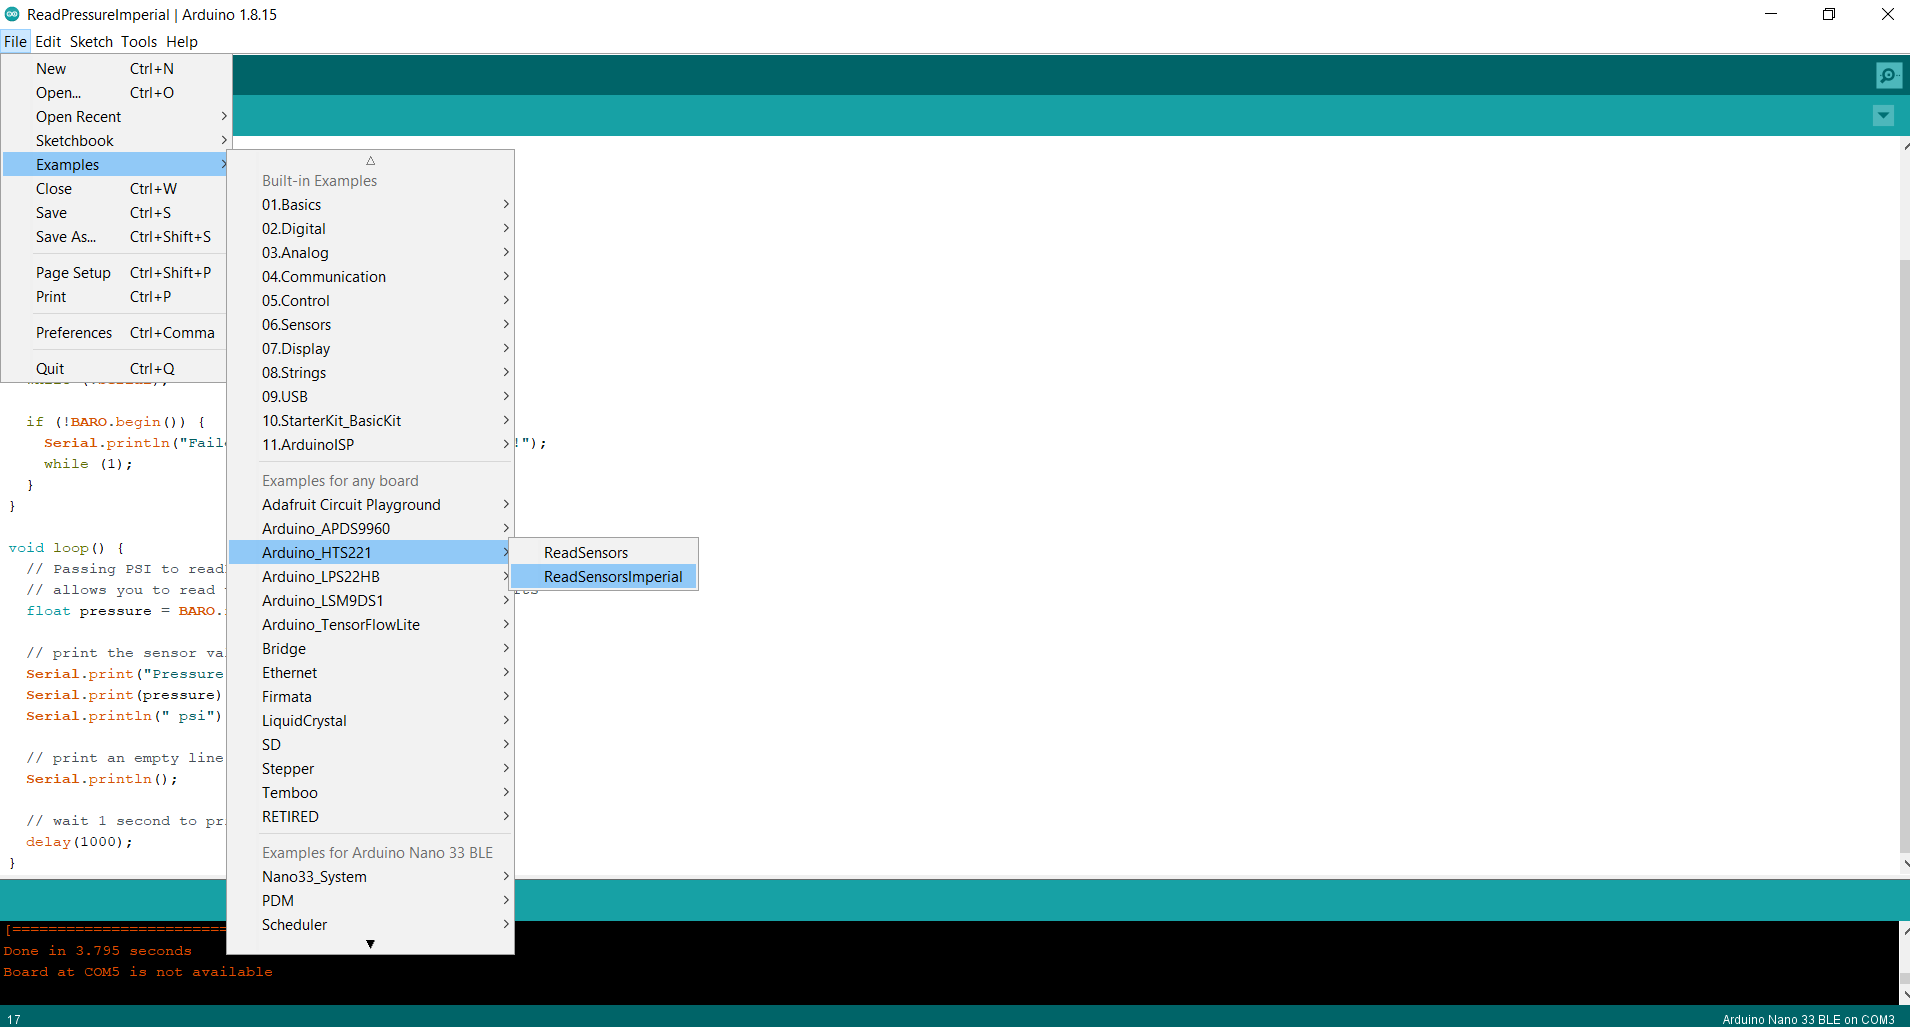
\includegraphics[width=8cm]{Nano33BLESense/7}
    \captionof{figure}{HTS221, Humidity and Temperature Sensor}
    \label{fig:5}
\end{center}

The on-board embed HTS221 sensor on Arduino Nano 33 BLE Sense has the funcnality to measure the relative humadity and temperature in the environment. The procedure for getting access to his library and code also the same as the other sensors have as shown in the figure.  \ref{fig:5}

After Uploading and compiling the program, the environmental humidity and temperature also display in the serial monitor as shown in the figure.  \ref{fig:6} By getting access to these values, change the port again after compiling the program for opening the serial monitor, these values help us to make the application with electrical appliances regarding energy savings or modify the code and add some external devices with the GPIO of Arduino Nano 33 BLE Sense too and control it as per the humidity and temperature values.

\begin{center}
    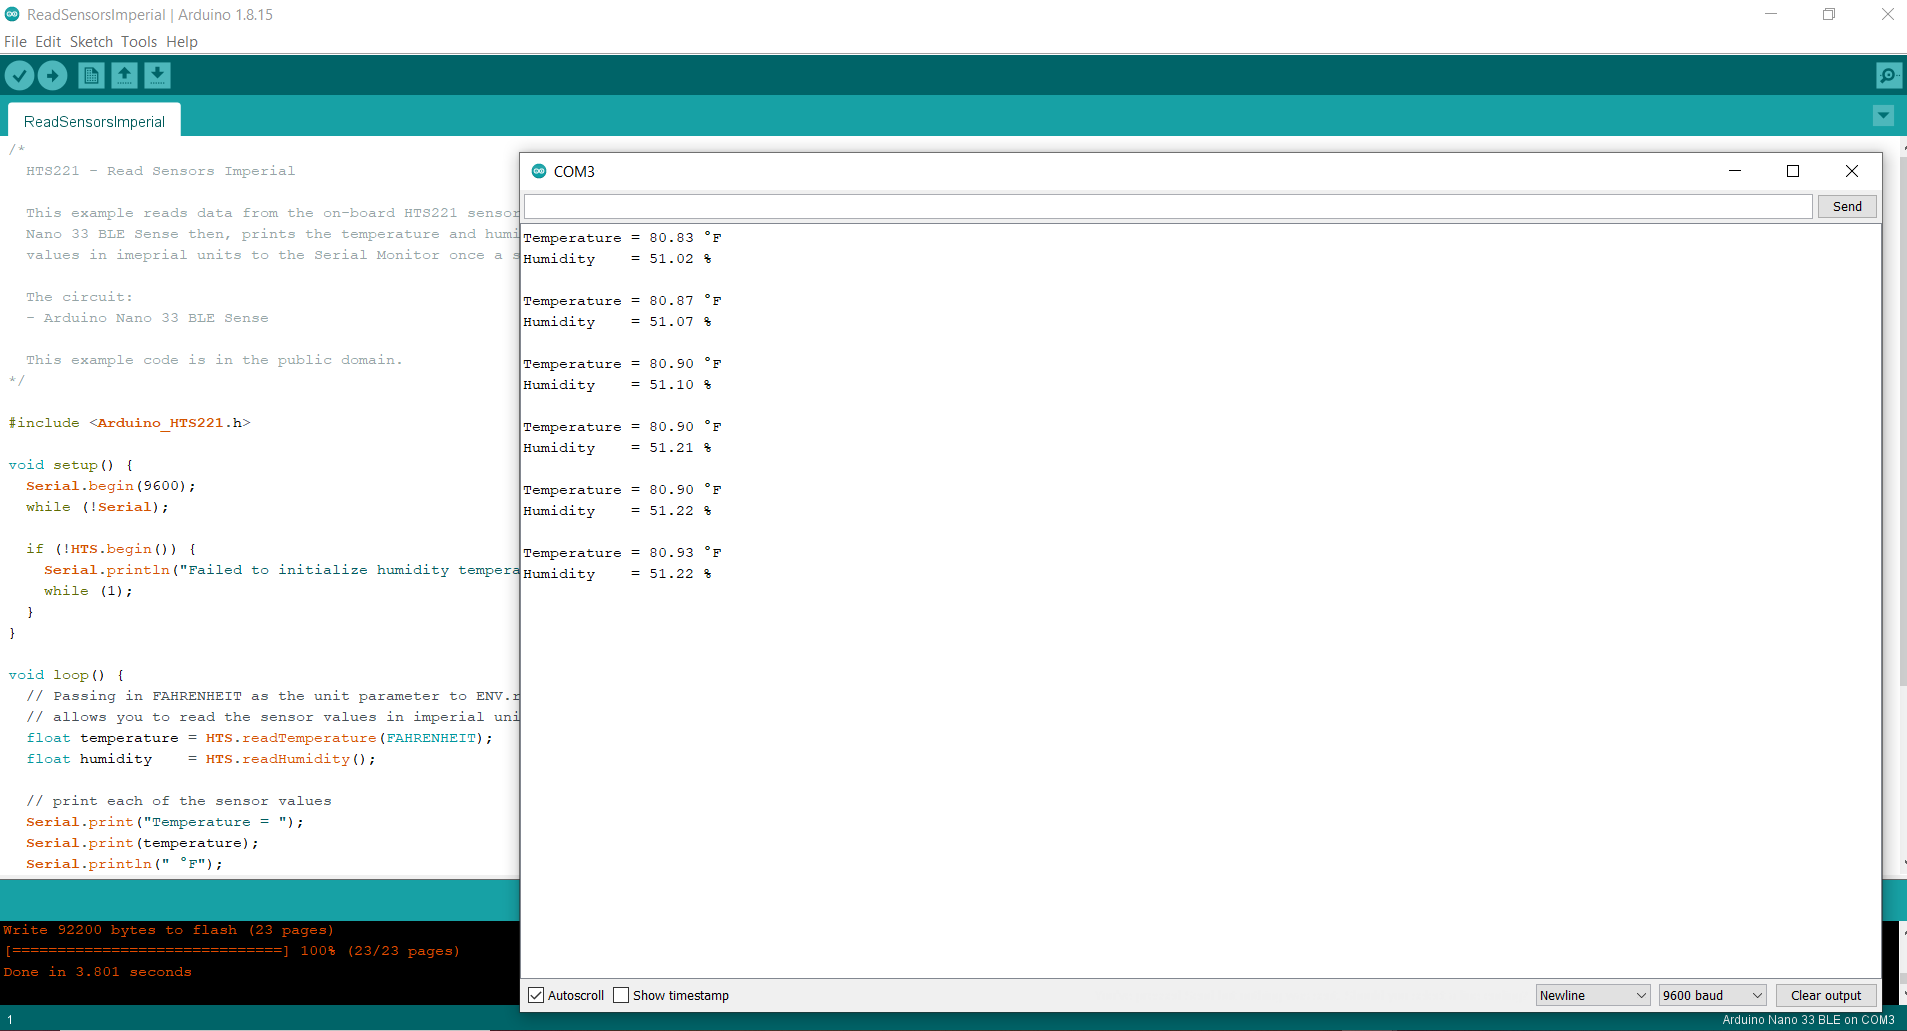
\includegraphics[width=8.5cm]{Nano33BLESense/8}
    \captionof{figure}{HTS221, Output Window}
    \label{fig:6}
\end{center}


\section{General}

General description

cite books

\section{Specific Sensor}

cite board

\section{Specification}

\begin{itemize}
  \item cite data sheet
  \item Circuit Diagram
\end{itemize}

\section{Bibliothek}

\subsection{Description}

\subsection{Installation}

\subsection{Functions}

\subsection{Example - Manual}

\subsection{Example}

\subsection{Example - Code}

\subsection{Example - Files}



\section{Calibration}

cite method

\section{Simple Code}


\section{Simple Application}



\section{Tests}

\subsection{Simple Function Test}

\subsection{Test all Functions}

\section{Simple Application}


\section{Further Readings}

